%\documentclass[10pt, a4paper]{article}

\documentclass[12pt]{article}

\usepackage{sbc-template}


% Pacotes essenciais para artigos da SBC
\usepackage[utf8]{inputenc}
\usepackage[T1]{fontenc}
\usepackage[portuguese]{babel} % Suporte a língua portuguesa
\usepackage{graphicx} % Para inserir imagens
\usepackage{booktabs}
\usepackage[hidelinks]{hyperref} % Para links
\usepackage{amsmath} % Pacote para equações (útil, mesmo se não for usar)
\usepackage{amssymb}
\usepackage{booktabs} % Para tabelas com linhas profissionais
%\usepackage[left=2.5cm, right=2.5cm, top=3cm, bottom=3cm]{geometry} % Margens padrão

% Redefine comandos para o formato de cabeçalho da SBC
\makeatletter
\renewcommand{\@author}[1]{\centerline{\sc #1}}
\renewcommand{\@date}[1]{}
\renewcommand{\@title}[1]{{\Large \bfseries \centerline{#1}}}
\makeatother

\usepackage{comment}
\usepackage{color}
%\usepackage{ifthen} 
% Removida a linha problemática \cl{...}

\newcommand{\cl}[1]{\textcolor{red}{\textbf{[Crescencio: #1]}}}

% Informações do artigo
\title{Da Operação Analógica ao Controle Computacional: \\Estudo de Caso da Transformação Digital da Cadeia de Frio em uma Empresa Avícola}
%Da Operação Analógica ao Controle Computacional: Um Estudo de Caso sobre a Implantação do Sistema Sitrad Pro em uma Empresa Avícola da Região}

\author{Sidnelson Gubert\inst{1}, Crescencio Rodrigues Lima Neto  \inst{1}}

\address{Instituto Federal de Educação, Ciência e Tecnologia da Bahia (IFBA)\\
45078-300 -- Vitória da Conquista -- BA -- Brasil
\email{\{sidgubert, crescencio\}@gmail.com}}

\begin{document}

\maketitle

\begin{abstract}
%This case study investigates the successful transition from an analog control system to a computational approach in the cold chain of an poultry company located in the region. Previously reliant on electromechanical equipment vulnerable to unmonitored failures, the company implemented the Sitrad Pro system, using TC900 and LOG control instruments connected to TCP 485 converters. This solution enabled real-time online monitoring and automation of the refrigeration park, encompassing 9 critical environments (2 Chambers, 3 Freezing Tunnels, and 4 Storage Containers). The results show that digital modernization provided complete operational visibility, mitigated product losses, and optimized the team's response capability. The study concludes that Refrigeration 4.0 and Industry 4.0 are intrinsically linked to the advancement of information and computer technology.

Food safety and product quality in the poultry industry depend on strict temperature control throughout the cold chain, especially during freezing and storage.  A company operated with an analog electromechanical control system characterized by reactive equipment, limited diagnostic capability, and high vulnerability to unmonitored failures. This scenario compromised operational reliability and increased the risk of product losses in critical refrigeration environments. This article presents a case study aimed at supporting the transition to an integrated computational control system, assessing its impacts on supervision, automation, and operational performance of the cold chain. The modernization was implemented through the adoption of the Sitrad Pro software, together with TC900 and LOG control instruments connected to TCP-485 converters. The system was deployed across nine environments—two cold rooms, three freezing tunnels, and four storage containers—enabling real-time monitoring and automation of the refrigeration infrastructure. The migration provided full operational visibility, allowing supervision of critical parameters and proactive response to anomalies. A reduction in product losses, greater thermal stability, and improved team performance were observed, as personnel began operating based on data and automated alerts.

\textbf{Keywords:} Automation, Industry 4.0, IoT, Cold Chain, Predictive Maintenance.

\end{abstract}

\begin{resumo} 

A segurança e a qualidade na avicultura dependem do controle térmico rigoroso durante o congelamento e o armazenamento na cadeia de frio.  Uma empresa avícola operava com um sistema de controle eletromecânico analógico, caracterizado por equipamentos reativos, baixa capacidade de diagnóstico e elevada vulnerabilidade a falhas não monitoradas. Esse cenário comprometia a confiabilidade operacional e aumentava o risco de perdas de produto em ambientes críticos de refrigeração. Este artigo apresenta um estudo de caso que teve como objetivo auxiliar na transição para um sistema de controle computacional integrado, avaliando seus impactos na supervisão, automação e desempenho operacional da cadeia de frio. A modernização foi implementada por meio da adoção do software Sitrad Pro, associado a instrumentos de controle TC900 e LOG conectados a conversores TCP-485. O sistema foi aplicado a nove ambientes — duas câmaras, três túneis de congelamento e quatro contêineres de armazenamento — possibilitando monitoramento em tempo real e automação do parque de refrigeração. A migração proporcionou visibilidade completa da operação, permitindo a supervisão dos parâmetros e a resposta proativa a anomalias. Observou-se redução das perdas de produto, maior estabilidade térmica e otimização da atuação da equipe, que passou a operar com base em dados e alertas automatizados.

\begin{comment}
Este estudo de caso investiga a transição bem-sucedida de um sistema de controle \textbf{eletromecânico (analógico)} para uma abordagem computacional na cadeia de frio de uma empresa avícola da região. Anteriormente dependente de equipamentos \textbf{reativos} e vulneráveis a falhas não monitoradas, a empresa implementou o sistema Sitrad Pro, utilizando instrumentos de controle TC900 e LOG conectados a conversores TCP 485. Essa solução permitiu o monitoramento **supervisionado** online em tempo real e a automação do parque de refrigeração, que envolve 9 ambientes críticos (2 Câmaras, 3 Túneis de Congelamento e 4 Contêineres de Armazenamento). Os resultados demonstram que a modernização digital proporcionou visibilidade completa da operação, mitigou \textbf{significativamente} perdas de produto e otimizou a capacidade de resposta da equipe. O estudo conclui que a Refrigeração 4.0 e a Indústria 4.0 estão intrinsecamente ligadas ao avanço da tecnologia da informação e da computação.
\end{comment}

\textbf{Palavras-Chave:} Automação, Indústria 4.0, IoT, Cadeia de Frio.

\end{resumo}

% Início do corpo do artigo
\section{Introdução}
%A segurança alimentar e a qualidade do produto final na indústria avícola dependem criticamente de um controle rigoroso da cadeia de frio, especialmente nas etapas de congelamento e armazenamento. A manutenção da temperatura ideal nas \textbf{duas Câmaras (A e C)}, nos \textbf{três Túneis de Congelamento (D, E e F)} e nos \textbf{quatro Contêineres de Armazenamento (1, 2, 3 e 4)} é um processo essencial, mas que historicamente enfrentava desafios significativos em modelos operacionais mais tradicionais. Em uma empresa avícola da região, o sistema de refrigeração, embora funcional, era majoritariamente baseado em componentes eletromecânicos, carecendo de um sistema de supervisão e controle remoto. O setor, no entanto, tem cada vez mais buscando modernizar suas operações, alinhando-se aos princípios da Indústria 4.0 \cite{tecnotri2019}.

A segurança alimentar e a qualidade do produto final na indústria avícola dependem diretamente da manutenção precisa das condições térmicas ao longo de toda a cadeia de frio, especialmente nas etapas de congelamento e armazenamento. Nessas fases, o controle adequado da temperatura em câmaras, túneis de congelamento e contêineres de estocagem constitui um requisito indispensável para a integridade do produto. 

Apesar disso, muitos processos ainda operam sob modelos tradicionais de refrigeração, nos quais a supervisão é limitada e a automação, incipiente. Esse era o caso de uma empresa avícola da região, cujo parque de refrigeração, embora funcional, era predominantemente composto por dispositivos eletromecânicos e desprovido de um sistema de monitoramento e controle remoto. Paralelamente, o setor avícola tem avançado em direção à modernização tecnológica, impulsionado pelos princípios da Indústria 4.0 \cite{tecnotri2019}, que demandam maior integração, inteligência operacional e conectividade.

%O principal problema dessa abordagem era a vulnerabilidade a falhas. Em períodos de menor atividade, como no meio da noite ou em feriados, a ocorrência de problemas nos túneis de congelamento passava despercebida por falta de acompanhamento humano. Essa carência de visibilidade e automação representava um risco considerável de \textbf{deterioração do produto} e perdas \textbf{financeiras} irreparáveis, comprometendo a qualidade e a segurança alimentar. Em resposta a esse desafio, a empresa buscou uma solução que permitisse transformar a infraestrutura existente, conferindo-lhe inteligência, conectividade e controle.

A fragilidade do modelo anterior tornava-se evidente em situações de baixa presença humana, como períodos noturnos e feriados. Nesses momentos, falhas em túneis de congelamento ou demais ambientes críticos podiam passar despercebidas, já que não havia meios de supervisão contínua. A ausência de visibilidade operacional representava um risco elevado de deterioração de produtos e perdas financeiras, impactando diretamente a segurança alimentar e a eficiência produtiva. Diante desse cenário, tornou-se evidente a necessidade de transformar a infraestrutura existente, incorporando recursos digitais capazes de ampliar o controle, aumentar a confiabilidade e antecipar problemas antes que se convertessem em prejuízos.

%A presente pesquisa tem como objetivo analisar a implantação do sistema Sitrad Pro como a ferramenta computacional escolhida para resolver o problema. O estudo de caso visa demonstrar como a integração de instrumentos de controle eletromecânicos (TC900 e LOG) com conversores de comunicação (TCP 485) tornou possível dar visibilidade total ao parque de refrigeração, permitindo o acompanhamento em tempo real e a automação do processo. Por meio da análise dos resultados, este artigo busca reforçar a relevância da computação para a modernização da indústria, alinhando a empresa com os princípios da Refrigeração e da Indústria 4.0.

Nesse contexto, este trabalho apresenta um estudo de caso que auxiliou na adoção de uma solução computacional integrada para superar as limitações do modelo tradicional de supervisão da cadeia de frio. O estudo evidencia como a integração entre instrumentos de controle eletromecânicos, dispositivos de registro e conversores de comunicação — conectados por meio de uma arquitetura digital baseada em protocolos industriais — possibilitou a implementação de uma plataforma de monitoramento em tempo real. Essa infraestrutura ampliou a visibilidade operacional do parque de refrigeração e permitiu a automação de processos críticos, antes dependentes de intervenção humana constante. A partir da avaliação dos resultados obtidos, o artigo demonstra o papel estratégico das tecnologias da computação na modernização da indústria avícola, fortalecendo sua convergência com os princípios da Refrigeração 4.0 e da Indústria 4.0.

% Nesse contexto, este trabalho apresenta um estudo de caso que teve como objetivo auxiliar na implantação do sistema Sitrad Pro como solução computacional adotada pela empresa para superar essas limitações. O estudo de caso demonstra como a integração de instrumentos de controle eletromecânicos (TC900 e LOG) com conversores de comunicação TCP-485 possibilitou a criação de uma plataforma de supervisão em tempo real, oferecendo visibilidade completa do parque de refrigeração e permitindo a automação de processos críticos. A partir da avaliação dos resultados obtidos, o artigo evidencia o papel central da computação na modernização da indústria avícola, reforçando sua convergência com os princípios da Refrigeração 4.0 e da Indústria 4.0.


O restante deste documento está estruturado da seguinte forma: Seção \ref{sec:referencial_teorico} apresenta o referencial teórico da pesquisa. A Seção \ref{sec:metodologia} detalha a metodologia aplicada na construção da solução. A Seção \ref{sec:resultados} apresenta a análise e discussão dos resultads. Por fim, a Seção \ref{sec:conclusao} explica as conclusões da pesquisa e sua limitações e fala sobre os trabalhos futuros.

\section{Revisão da Literatura} \label{sec:referencial_teorico}

A Indústria 4.0, frequentemente referida como a Quarta Revolução Industrial, representa uma transformação na forma como os produtos são fabricados, distribuídos e controlados. Ela se concentra na digitalização e na interconexão de sistemas de produção e é caracterizada pela integração de tecnologias como a Internet das Coisas (IoT), sistemas ciberfísicos, computação em nuvem, \textit{big data} e inteligência artificial (IA) \cite{RIFFAI_2022}.

No contexto da indústria de alimentos e, em particular, na agroindústria avícola, a aplicação da Indústria 4.0 é crucial para garantir a rastreabilidade, segurança e eficiência produtiva \cite{JARDIM_2023}. A automação de processos e a coleta de dados em tempo real permitem um controle mais preciso sobre a produção. A adoção desses princípios na cadeia de controle climático de ambientes fechados, como os galpões de aves, é o que garante a zona de conforto térmico ideal para maximizar o desempenho zootécnico e o bem-estar animal \cite{TINOCO_2011}.

\subsection{Internet das Coisas (IoT) no Controle Ambiental Avícola}

A IoT é um pilar central da Indústria 4.0 e desempenha um papel fundamental na modernização dos sistemas de climatização. A IoT permite que dispositivos físicos, como sensores de temperatura e controladores, sejam conectados à internet e se comuniquem uns com os outros e com sistemas de gestão centralizados. Essa conectividade transforma equipamentos passivos em fontes de dados ativas e em pontos de controle remotos.

Na empresa, a implementação do sistema Sitrad Pro representa um caso prático da IoT. Os controladores de temperatura (TC900 e LOG) atuam como "coisas" inteligentes que coletam dados e executam comandos, enquanto o conversor TCP 485/04 serve como o \textit{gateway} de comunicação que os conecta à nuvem. Essa arquitetura possibilita o monitoramento contínuo e a intervenção remota, sendo fundamental na transição de um sistema reativo para um sistema digital e proativo. A capacidade de coletar e analisar dados em tempo real é o cerne da Zootecnia de Precisão, permitindo a otimização de processos e a minimização do estresse térmico, impactando diretamente a qualidade do lote e a conversão alimentar \cite{ABREU_2016}.

\subsection{Manutenção Preditiva e Impacto na Eficiência Operacional}

A transição de um modelo de manutenção reativo para um preditivo é um dos maiores benefícios da Indústria 4.0. A Manutenção Preditiva (MP) utiliza a coleta e análise contínua de dados em tempo real (como temperatura, corrente elétrica, ciclos de trabalho) para prever a ocorrência de falhas em equipamentos antes que elas se manifestem \cite{ABDELSALAM_2024}. Diferentemente da manutenção preventiva, que atua em intervalos fixos, a MP otimiza o tempo de intervenção, minimizando o tempo de inatividade não planejado, reduzindo custos de manutenção e aumentando a vida útil do sistema \cite{CAMPOS_SILVA_2021}.

No contexto da empresa, o monitoramento contínuo dos controladores (TC900 e LOG) pelo Sitrad Pro estabelece a base para a MP. Ao analisar as tendências de parâmetros – por exemplo, um tempo excessivo de acionamento do motor de ventilação para atingir a temperatura ideal, ou variações anômalas de leitura – o sistema é capaz de identificar anomalias que possam indicar um problema iminente em exaustores, \textit{coolings} ou aquecedores \cite{baldissarelli2019}. Essa detecção precoce de desvios operacionais é essencial para a avicultura, pois permite que a equipe intervenha e evite a interrupção da operação crítica e a subsequente perda de produtos (aves) causada por estresse térmico agudo \cite{NAAS_2007}. A MP, portanto, transforma um processo de controle reativo em um sistema de gestão proativo e preditivo.

No caso da empresa, o monitoramento contínuo dos controladores TC900 e LOG pelo Sitrad Pro permite que a equipe identifique anomalias nos ciclos de congelamento ou nos parâmetros de temperatura que possam indicar um problema iminente. Essa capacidade de detecção precoce de desvios operacionais representa uma mudança de paradigma, saindo de um cenário onde os problemas eram descobertos apenas após a ocorrência de uma perda, para um cenário onde a equipe pode intervir e evitar a interrupção da operação e a perda de produtos.

\section{Metodologia} \label{sec:metodologia}

\subsection{Justificativa Tecnológica: A Resposta à Refrigeração 4.0}

O presente estudo se configura como um Estudo de Caso de caráter comparativo, detalhando a metodologia de implementação de um sistema de automação em ambientes de refrigeração industrial e mensurando seu impacto. O projeto na empresa foi concebido como uma resposta estratégica à Refrigeração 4.0 (a aplicação dos princípios da Indústria 4.0 na cadeia de frio), visando a migração de um controle reativo para um sistema de gestão preditivo e conectado. O ponto de partida foi a necessidade crítica de otimizar a estabilidade térmica e a rastreabilidade nos 9 ambientes críticos: Câmaras A e C, Túneis de Congelamento D, E, F e Contêineres de Armazenamento 1, 2, 3 e 4.

\subsection{Arquitetura do Sistema e Instrumentos}

O sistema de refrigeração da empresa, em sua configuração anterior, baseava-se em uma arquitetura de controle analógica e eletromecânica. Neste modelo, cada controlador (TC900 ou LOG) operava como uma unidade de controle isolada, dependendo de medições pontuais e da inspeção humana para detecção de anomalias.

A modernização introduziu a arquitetura de Refrigeração 4.0, onde o novo sistema utiliza os controladores Full Gauge existentes, mas os integra a um barramento de comunicação RS-485, que se conecta a um servidor centralizado via IoT. Essa nova disposição converte o controle isolado em um sistema supervisionado e preditivo.

\subsection{Planejamento e Execução do Projeto}

O projeto de modernização tecnológica da empresa foi conduzido em alinhamento com as boas práticas de Gerenciamento de Projetos, seguindo as etapas dos Grupos de Processos (Iniciação, Planejamento, Execução, Monitoramento e Controle, e Encerramento) definidas pelo \textit{Project Management Institute} (PMI) \cite{pmbok2021}. Dada a natureza do projeto – implementação de um sistema de informação e automação – foi crucial abordar o planejamento de forma sistêmica, reconhecendo a interdependência entre a instalação física e a configuração lógica \cite{kerzner2015}.

\subsection{Materiais Utilizados}

\begin{itemize}
    \item 01 - Servidor Lenovo Thinksystem St50 Xeon E-2224g 4c Hd 1tb 8gb - Windows Server 2016
    \item 01 - Conversor TCP-485 da Full Gauge
    \item 09 - Controlador p Refrigeração 115/230V Tc900e Log Full Gauge
    \item 200 metros de cabo Cat6 (Categoria 6)
\end{itemize}

\subsubsection{Planejamento Detalhado}

A fase de Planejamento \cite{pmbok2021} estabeleceu as diretrizes para a execução, focando em quatro pilares críticos:

\begin{enumerate}
    \item \textbf{Justificativa e Escolha Tecnológica:} A seleção da \textit{Full Gauge Controls} e, em particular, dos instrumentos TC900 e LOG, foi um ponto central do planejamento, pautado na relação custo-benefício e na adequação ao ambiente industrial avícola.
    \begin{itemize}
        \item \textbf{Custo e Disponibilidade:} Os instrumentos da \textit{Full Gauge} são amplamente distribuídos e possuem um custo de aquisição e reposição competitivo no mercado nacional. Sua disponibilidade minimizou o risco de atraso na aquisição de hardware.
        \item \textbf{Confiabilidade e Modularidade:} Os controladores (TC900 e LOG) possuem um histórico comprovado de confiabilidade em refrigeração industrial e a capacidade de se integrar em rede (protocolo RS-485), garantindo a escalabilidade e a comunicação de múltiplas unidades de frio.
        \item \textbf{Funcionalidades de Qualidade:} O software Sitrad Pro oferece registro histórico automatizado (\textit{data logging}) e emissão de relatórios de conformidade, necessários para atender às exigências de segurança alimentar e auditoria.
    \end{itemize}
    \item \textbf{Definição do Escopo e Qualidade:} O escopo foi definido como a centralização do monitoramento dos nove controladores de temperatura do parque frigorífico, abrangendo os nove ambientes. A qualidade foi definida pela garantia de disponibilidade de dados (99\%)} e pela precisão das leituras de temperatura em tempo real.
    \item \textbf{Gestão de Recursos e Riscos:} Foram alocados recursos de infraestrutura (servidor dedicado e infraestrutura de rede) e humanos (equipe de Tecnologia da Informação (TI), técnicos de manutenção e especialista em automação). Os riscos, como a estabilidade da rede de comunicação e o potencial tempo de inatividade durante a instalação dos conversores RS-485, foram mapeados e mitigados através de testes prévios e agendamento das intervenções para períodos de menor carga operacional (produção reduzida ou pausas).
    \item \textbf{Cronograma e Comunicação:} Foi estabelecido um cronograma em fases, priorizando a interligação da rede RS-485 e a instalação física dos conversores, seguida pela configuração do software. O Plano de Comunicação garantiu que a equipe de Manutenção, Produção e a alta gestão fossem informadas sobre o progresso e os eventuais desvios.
\end{enumerate}

\subsubsection{Execução e Configuração do Sistema}

A Execução envolveu a mobilização dos recursos e a materialização do projeto. As principais atividades realizadas foram:

\begin{enumerate}
    \item \textbf{Instalação de Campo e Infraestrutura:} A rede de comunicação serial RS-485, responsável pela coleta de dados, foi instalada em um layout de barramento. Em cada câmara, foram instalados os conversores RS-485, responsáveis por interligar os controladores à rede local de dados (Ethernet/TCP-IP), conforme o diagrama de instalação proposto (Figura \ref{fig:esquema_instalacao}).
    \item \textbf{Configuração do Servidor Sitrad Pro:} O software Sitrad Pro foi instalado no servidor dedicado, centralizando o banco de dados. Foi realizada a configuração individual de cada um dos 9 controladores, incluindo a parametrização de seus endereços de comunicação (\textit{polling}) e a criação de telas de visualização personalizadas para cada setor da fábrica.
    \item \textbf{Validação e Treinamento (\textit{Go-Live}):} Após a configuração, o sistema foi operado em paralelo ao método manual por um período de teste (\textit{burn-in period}). A precisão dos dados e o funcionamento dos alertas foram validados junto à equipe de Manutenção. O treinamento operacional foi fornecido para garantir a utilização correta do sistema de monitoramento e a interpretação dos alarmes de temperatura e falha, garantindo a sustentabilidade da solução \cite{saviani2024}.
\end{enumerate}


Figura \ref{fig:esquema_instalacao} apresenta o esquema físico de interligação entre os controladores de temperatura, os módulos de ligação da rede RS-485 e o conversor TCP-485, responsável por integrar o sistema de refrigeração ao software Sitrad PRO, instalado em um computador ou servidor. O Sitrad PRO se comunica com o conversor TCP-485, recebendo os dados dos controladores e exibindo informações como temperatura, alarmes e registros históricos. O conversor TCP-485 (WiFi/LOG) converte os sinais da rede RS-485 para o protocolo TCP/IP, permitindo que o computador acesse os dados via rede local ou internet. Cada controlador TC-900/LOG mede temperatura, aciona compressores/ventiladores e envia os valores ao barramento RS-485.

\begin{figure}[!ht]
    \centering
    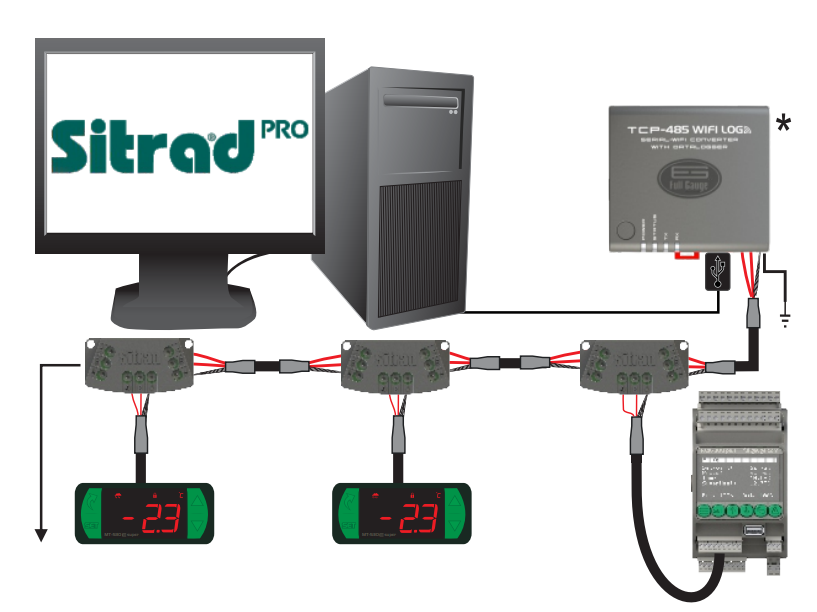
\includegraphics[width=\columnwidth]{esquema_instalacao.png}
    \caption{Esquema Físico de Interligação dos Controladores e Conversores TCP 485/04 (Adaptado de Full Gauge Controls).}
    \label{fig:esquema_instalacao}
\end{figure}

\begin{comment}
\begin{table}[h]
    \centering
    \caption{Planejamento de Execução do Projeto de Automação}
    \label{tab:planejamento}
    \begin{tabular}{|p{0.18\linewidth}|p{0.2\linewidth}|p{0.5\linewidth}|} 
        \hline
        \textbf{Fase} & \textbf{Período Estimado} & \textbf{Atividades-Chave} \\
        \hline
        I. Planejamento & Jan/2023 & Levantamento de requisitos e infraestrutura. Definição e compra dos \textit{gateways} (TCP 485/04) e controladores digitais. \\
        \hline
        II. Instalação Física & Fev-Mar/2023 & Instalação dos controladores (ex: TC-900E Log) nos painéis. Cabeamento da rede RS-485 e sensores de temperatura nas câmaras. \\
        \hline
        III. Configuração & Abr/2023 & Interligação dos controladores ao conversor. Configuração de rede e instalação do software Sitrad Pro no servidor. \\
        \hline
        IV. Validação & Mai-Jun/2023 & Período de testes de campo para garantir a precisão do controle de temperatura em faixas críticas (por exemplo, $-18^\circ\text{C}$). Treinamento das equipes. \\
        \hline
    \end{tabular}
\end{table}
\end{comment}

A Tabela \ref{tab:planejamento} apresenta o planejamento de execução do projeto de automação da cadeia de frio, organizado em quatro fases sequenciais, cada uma com seu período de realização e atividades específicas. Na Fase I – Planejamento (Jan/2023), foram conduzidos o levantamento dos requisitos técnicos e da infraestrutura existente, além da definição e aquisição dos \texit{gateways} TCP 485/04 e dos controladores digitais necessários ao sistema.

A Fase II – Instalação (Fev–Mar/2023) envolveu a montagem física dos controladores — como os modelos TC-900E Log — nos painéis elétricos, assim como o cabeamento da rede RS-485 e a instalação dos sensores de temperatura nas câmaras frias. Na Fase III – Configuração (Abr/2023), ocorreu a interligação dos controladores ao conversor de comunicação, seguida da configuração da rede e da instalação do software de supervisão no servidor.

Por fim, a Fase IV – Validação (Mai–Jun/2023) consistiu em testes de campo para verificar a precisão do controle térmico em condições críticas, incluindo temperaturas da ordem de –18 °C, além do treinamento das equipes responsáveis pela operação do sistema.

\begin{table}[h]
    \centering
    \caption{Planejamento de Execução do Projeto de Automação}
    \label{tab:planejamento}
    \begin{tabular}{p{0.2\linewidth} p{0.18\linewidth} p{0.5\linewidth}}
        \toprule
        \textbf{Fase} & \textbf{Período} & \textbf{Atividades} \\
        \midrule
        I. Planejamento & Jan/2023 & Levantamento de requisitos e infraestrutura. Definição e compra dos \textit{gateways} (TCP 485/04) e controladores digitais. \\
        II. Instalação & Fev--Mar/2023 & Instalação dos controladores (ex.: TC-900E Log) nos painéis. Cabeamento da rede RS-485 e sensores de temperatura nas câmaras. \\
        III. Configuração & Abr/2023 & Interligação dos controladores ao conversor. Configuração de rede e instalação do software Sitrad Pro no servidor. \\
        IV. Validação & Mai--Jun/2023 & Período de testes de campo para garantir a precisão do controle de temperatura em faixas críticas (por exemplo, $-18^\circ\text{C}$). Treinamento das equipes. \\
        \bottomrule
    \end{tabular}
\end{table}


\section{Análise e Discussão dos Resultados} \label{sec:resultados}
%A implantação de uma solução computacional representou uma verdadeira transformação estratégica na gestão da sua cadeia de frio. A transição de um modelo de operação analógico e propenso a falhas para um sistema digitalmente integrado e supervisionado gerou impactos profundos e mensuráveis em diversas frentes operacionais. Os resultados obtidos solidificam a tese de que a Refrigeração 4.0, impulsionada pela computação e IoT, é fundamental para a competitividade e sustentabilidade na indústria avícola moderna.

A adoção de uma solução computacional representou uma transformação estratégica na gestão da cadeia de frio da empresa. A migração de um modelo analógico, limitado e suscetível a falhas, para uma arquitetura digital integrada e supervisionada em tempo real produziu impactos significativos e mensuráveis em múltiplas dimensões operacionais. Os resultados consolidados reforçam que a Refrigeração 4.0 — viabilizada por tecnologias de computação, conectividade e IoT — constitui um pilar essencial para a competitividade, a eficiência e a sustentabilidade da indústria avícola contemporânea.

\subsection{Visibilidade Operacional e Monitoramento em Tempo Real}
Um dos avanços mais significativos foi a aquisição de visibilidade operacional completa e em tempo real sobre o parque de refrigeração. Anteriormente, a dependência de verificações manuais ou a detecção tardia de problemas gerava um cenário de incerteza e alto risco. Com o Sitrad Pro, os instrumentos TC900 e LOG, atuando como sensores inteligentes conectados via TCP 485/04, passaram a alimentar o sistema com um fluxo contínuo de dados de temperatura, umidade e status de degelo (conforme ilustrado na Figura \ref{fig:figura2}).

Essa conectividade, alinhada aos princípios da IoT, permitiu à equipe de TI e manutenção monitorar cada ambiente remotamente, 24 horas por dia, abrangendo as câmaras, túneis e contêineres. A interface gráfica do Sitrad Pro oferece um painel de controle intuitivo que exibe instantaneamente qualquer desvio dos parâmetros configurados. Esta capacidade transformou a operação de um ciclo reativo — onde falhas eram descobertas após perdas significativas — para um ciclo proativo, onde as condições são supervisionadas ativamente. %Essa mudança é o cerne da **Zootecnia de Precisão** aplicada à ambiência do produto final.

\begin{figure}[!ht]
    \centering
    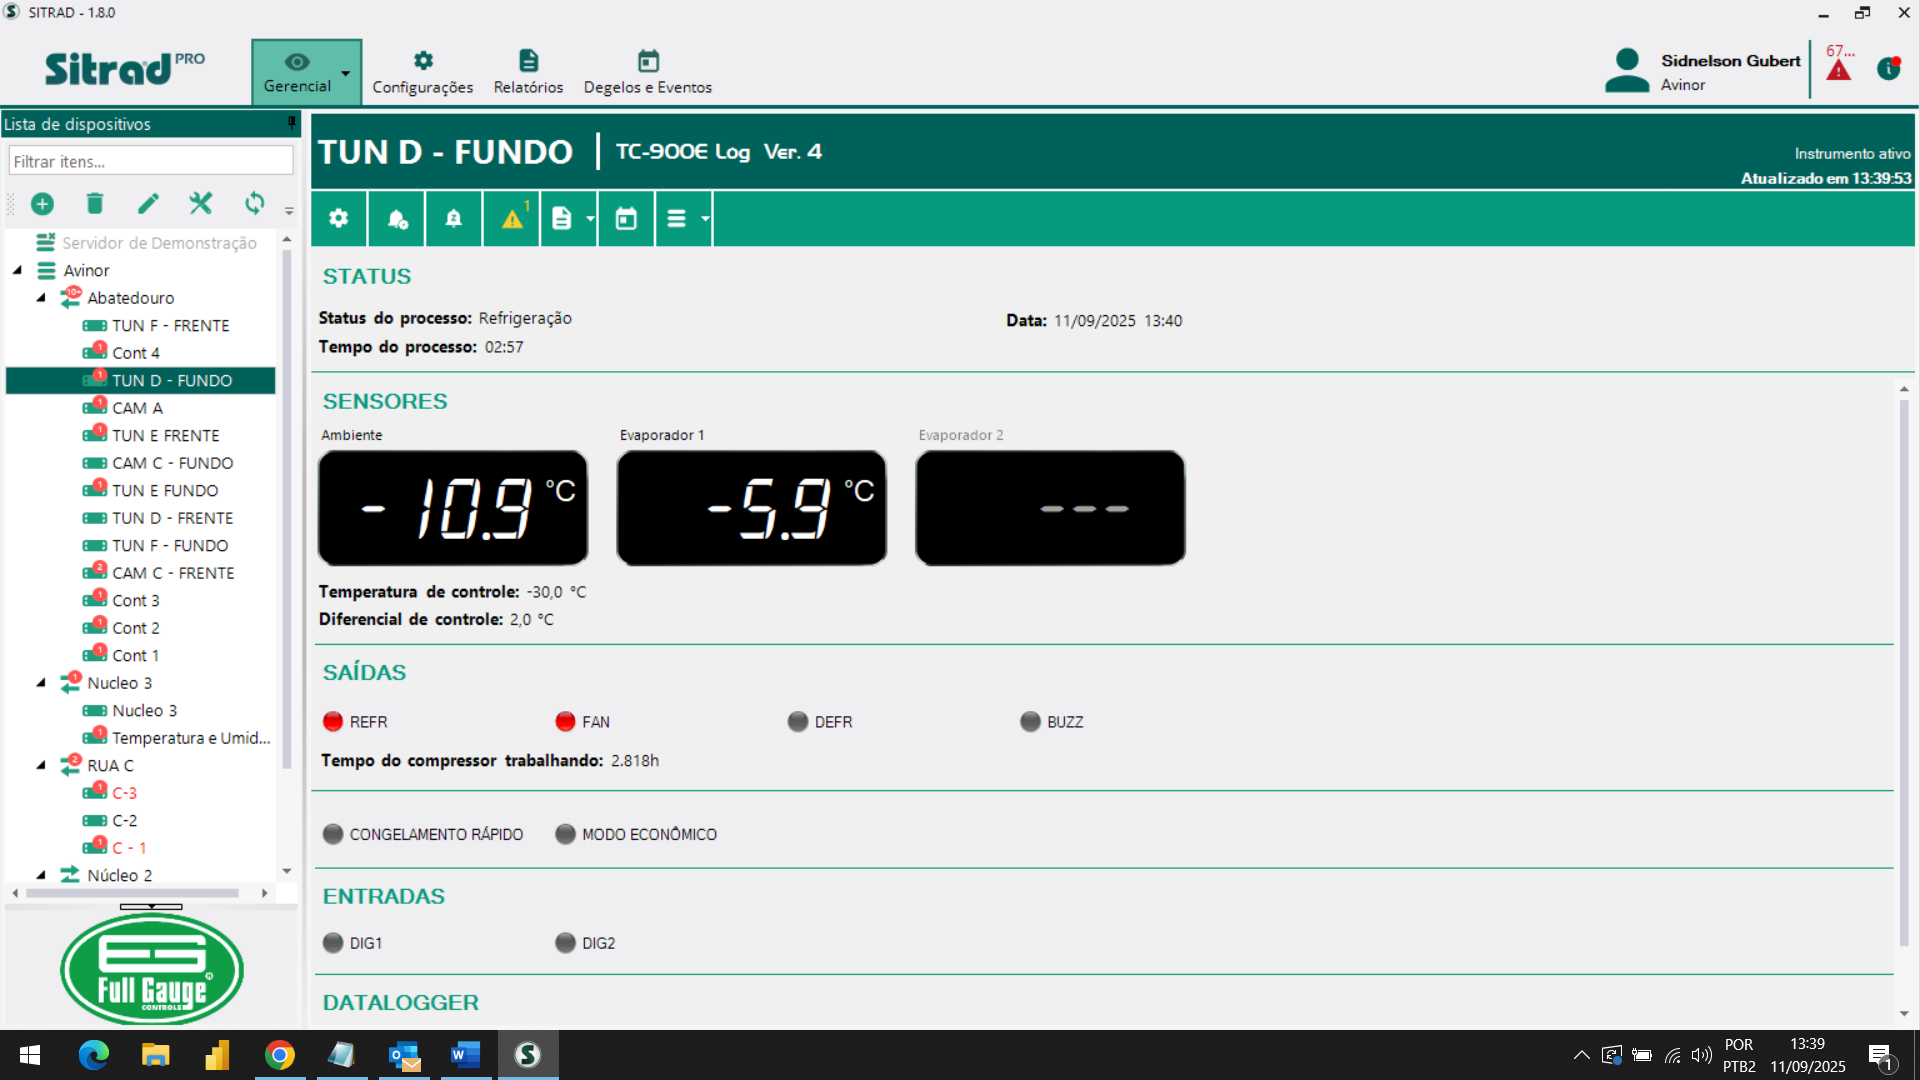
\includegraphics[width=\columnwidth]{figura2.png}
    \caption{Interface Gráfica do Sitrad Pro, Exibindo o Status em Tempo Real dos Controladores.}
    \label{fig:figura2}
\end{figure}

\subsection{Otimização da Manutenção e Prevenção de Perdas (Manutenção Preditiva)}
A visibilidade em tempo real se traduziu diretamente em uma otimização sem precedentes da manutenção e na prevenção de perdas de produto. Em regimes operacionais antigos, uma falha em um túnel de congelamento durante a noite ou em feriados poderia passar despercebida por horas, resultando na descongelação de grandes volumes de aves e, consequentemente, em perdas financeiras substanciais e riscos à segurança alimentar.

Com o novo sistema, o Sitrad Pro implementa um sistema de alertas e notificações automáticas. Quando as temperaturas se desviam dos padrões estabelecidos, alarmes sonoros, notificações via aplicativo móvel e e-mails são enviados instantaneamente aos gestores de manutenção. Essa capacidade de resposta imediata permitiu à equipe intervir rapidamente, minimizando o tempo de inatividade dos equipamentos e, crucialmente, salvaguardando a integridade dos produtos. A Figura \ref{fig:figura3} demonstra a capacidade de gerar relatórios detalhados, permitindo uma análise profunda das variações de temperatura e auxiliando na identificação de padrões que podem indicar a necessidade de manutenção preditiva \cite{zaro2023}. A análise desses dados históricos e em tempo real permite não apenas a correção de problemas, mas também a previsão de potenciais falhas em compressores ou ventiladores (seguindo o princípio de MP \cite{baldissarelli2019}), prolongando a vida útil dos equipamentos e otimizando os ciclos de degelo e congelamento.

\begin{figure}[h]
\centering
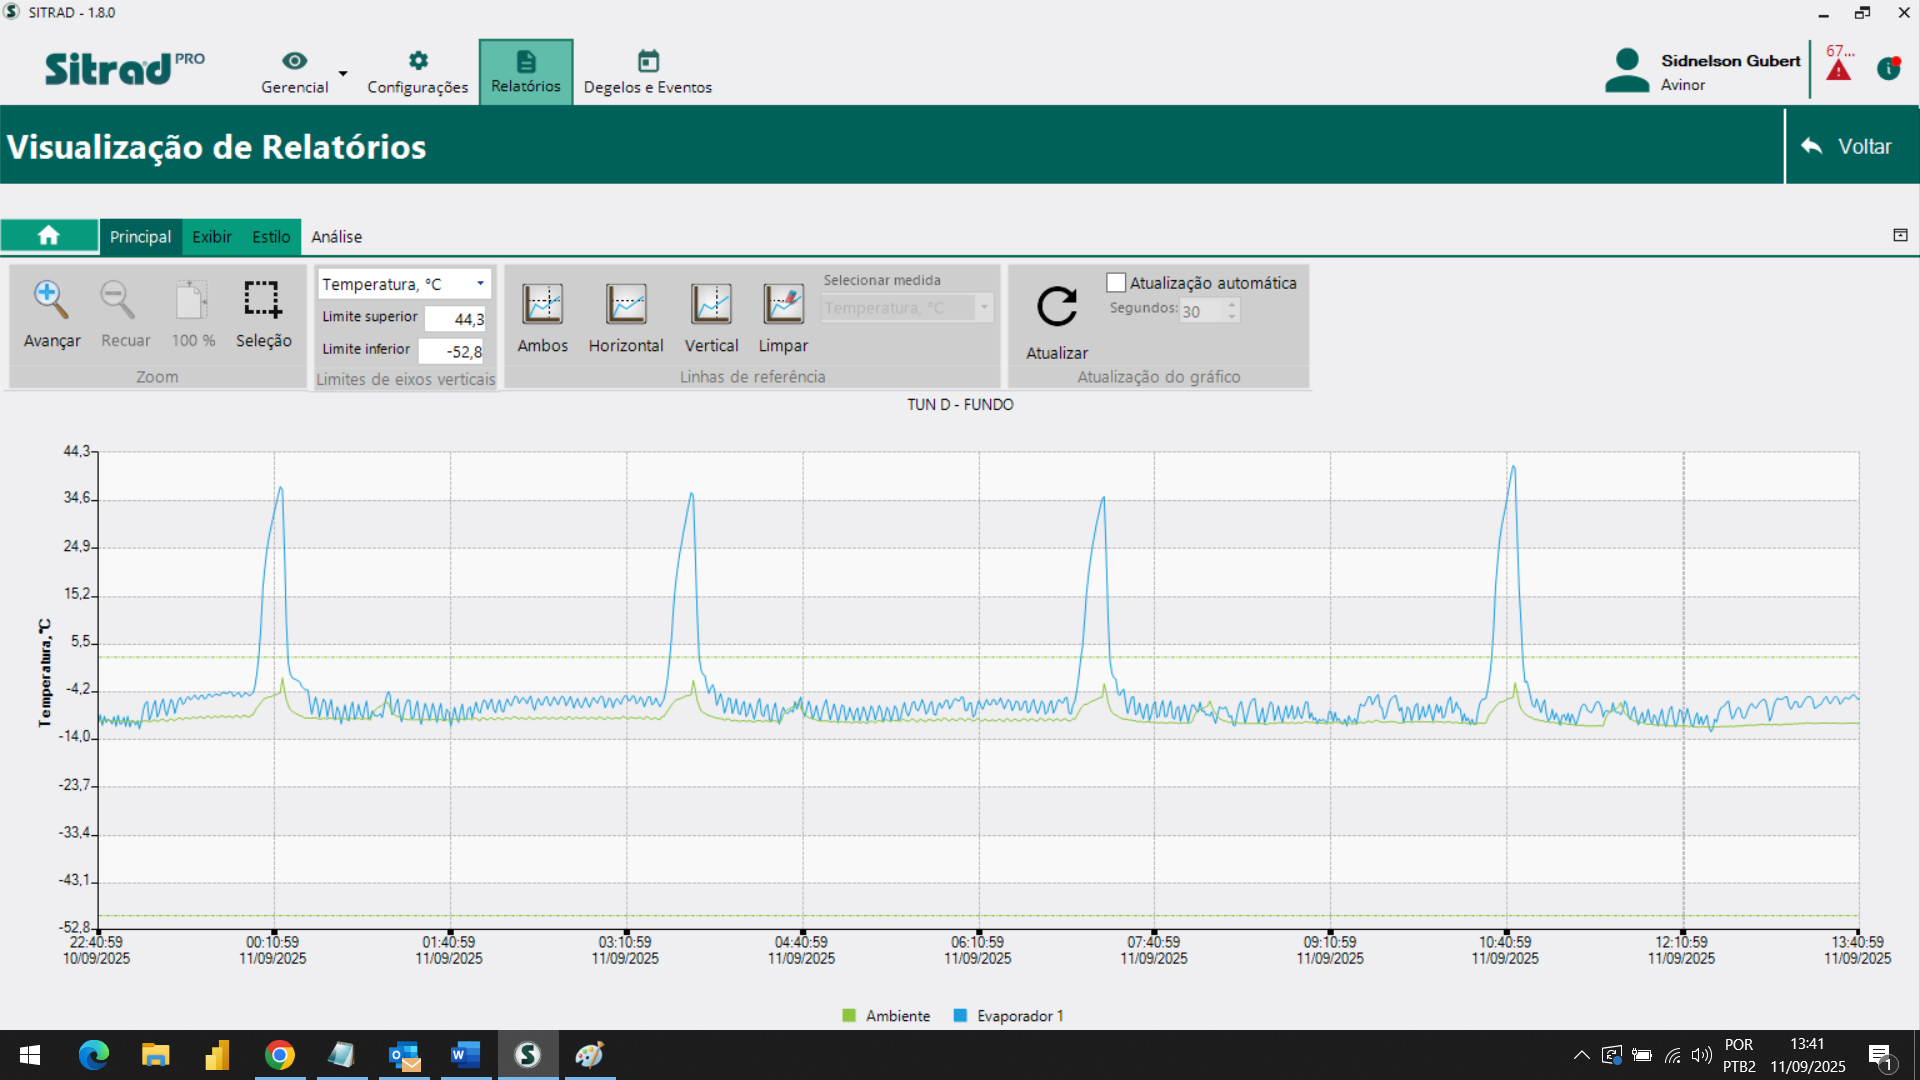
\includegraphics[width=1\textwidth]{figura3.png} % Certifique-se de que a imagem está no seu projeto
\caption{Exemplo de relatório de variação de temperatura. O gráfico exibe a variação de temperatura de um túnel de congelamento ao longo do tempo, permitindo à equipe de manutenção analisar o ciclo de congelamento e identificar padrões ou anomalias.}
\label{fig:figura3}
\end{figure}

\subsection{Tomada de Decisão Estratégica e Alinhamento com a Indústria 4.0}
Além dos benefícios operacionais diretos, a implantação da solução tecnológica elevou a capacidade de tomada de decisão estratégica na empresa. Com o acesso facilitado a dados confiáveis e em tempo real via aplicativo móvel, gestores de diferentes departamentos — manutenção, produção e comercial — agora podem acompanhar as condições da cadeia de frio a qualquer momento e de qualquer lugar.

Para a gestão de produção, a certeza de que os produtos estão sendo congelados nos tempos e temperaturas corretos permite um planejamento mais eficaz e a identificação de gargalos. Para o setor comercial, a visibilidade sobre a disponibilidade dos produtos na temperatura ideal otimiza a logística de expedição e a promessa de entrega. Essa integração de informações e a descentralização do acesso (com controle de perfis) é um pilar da Indústria 4.0, promovendo uma cultura organizacional baseada em dados e na colaboração interdepartamental.

A experiência da empresa demonstra que a Refrigeração 4.0 não é apenas uma automação de tarefas, mas uma integração holística que conecta o chão de fábrica à gestão estratégica, resultando em maior eficiência, redução de custos operacionais, aumento da segurança alimentar e, em última instância, maior competitividade no mercado. O sucesso do projeto valida a importância fundamental da tecnologia da informação e da computação como catalisadores da modernização industrial.

A integração dos componentes eletromecânicos com o sistema computacional demonstra que a Refrigeração 4.0 não é um conceito teórico, mas uma realidade prática que conecta o mundo físico ao digital, consolidando a importância da computação para a modernização e a competitividade da indústria avícola.

\subsection{Ameaças a validade}

As ameaças a validade do estudo podem ser organizadas em quatro dimensões: validade interna, validade externa, validade de construção e validade de conclusão.
Como o estudo utiliza um único caso, não há comparação com outras empresas ou com um cenário paralelo sem intervenção. Assim, é difícil afirmar que as melhorias observadas resultam exclusivamente da solução computacional e não de outros fatores, como mudanças organizacionais, capacitação de funcionários ou melhorias físicas na infraestrutura.

A empresa analisada possui um porte, layout, cultura organizacional e infraestrutura de refrigeração específicos. Portanto, os resultados podem não ser diretamente transferíveis para empresas maiores, menores ou com outra configuração tecnológica. Além disso, embora a descrição do sistema seja técnica, o estudo ainda depende de componentes específicos (TC900, LOG, TCP 485/04 e Sitrad Pro). Outras soluções tecnológicas podem produzir resultados diferentes, limitando a generalização para “Refrigeração 4.0” como um todo.


Os resultados enfatizam visibilidade, resposta a alarmes e redução de perdas, mas não quantificam métricas como tempo médio de falha (MTBF), tempo de resposta ou redução exata de perdas. Sem medidas objetivas, há risco de interpretar melhorias subjetivas como resultados comprovados.


Amostra limitada a um único período de operação. Os resultados podem ter sido influenciados por condições favoráveis durante o período analisado. A ausência de um acompanhamento de longo prazo reduz a confiança na estabilidade dos efeitos. Além disso, destaca-se a ausência de análise estatística. Sem dados quantitativos robustos, as conclusões dependem majoritariamente de observações qualitativas, o que reduz a confiabilidade do impacto real da solução computacional.

\section{Considerações Finais} \label{sec:conclusao}
A análise da implantação do sistema Sitrad Pro na empresa demonstra a bem-sucedida transição de um modelo de operação reativo para um sistema proativo e digitalmente integrado. Ao conectar componentes eletromecânicos a uma plataforma de monitoramento computacional e online, o projeto não apenas resolveu o problema de falhas não monitoradas, mas também gerou uma série de benefícios operacionais e estratégicos em toda a empresa.

Os resultados comprovam que a visibilidade em tempo real e a automação trouxeram maior segurança ao processo de congelamento, mitigando o risco de perdas de produto acabado e otimizando a capacidade de resposta da equipe. A inclusão de funções de notificação para temperaturas fora dos padrões esperados assegurou que qualquer anomalia seja imediatamente comunicada, permitindo intervenções rápidas e eficazes. Mais do que isso, a centralização e a acessibilidade dos dados, facilitada pelo aplicativo móvel, empoderaram diferentes setores da organização: a gestão de manutenção passou a acompanhar o desempenho dos equipamentos em tempo real, permitindo ações preditivas; a gestão de produção agora se baseia em dados confiáveis para se organizar; e o próprio setor comercial consegue prever com precisão os produtos que estarão disponíveis para expedição, otimizando a logística e o atendimento ao cliente. A manutenção da temperatura é crucial para a segurança alimentar, conforme as diretrizes da Agência Nacional de Vigilância Sanitária \cite{anvisa2004}, e o novo sistema garante que a empresa cumpra essa premissa.

O caso da empresa serve como um modelo exemplar de como a computação é o pilar central para a concretização dos princípios da Refrigeração 4.0 e da Indústria 4.0. A integração de hardware e software não é apenas uma melhoria tecnológica, mas uma ferramenta estratégica que transforma processos, organiza a gestão e assegura a competitividade no mercado. Este estudo de caso reforça a tese de que investir em sistemas de informação é fundamental para o futuro da indústria, tornando a operação mais inteligente, segura e eficiente.

Com sugestão de trabalhos futuros, seria interessante implementar controle automatizado baseado em IA. A partir da análise de padrões térmicos e operacionais, o sistema pode sugerir ou até aplicar automaticamente ajustes de temperatura, ciclos de degelo, ou regimes de operação mais eficientes. Estudos futuros podem investigar o uso de sensores redundantes ou autocalibráveis para aumentar a robustez do monitoramento e reduzir falsos positivos/negativos. Por fim, seria interessante criar modelos virtuais (implementação de gêmeos digitais (\textit{digital twins})) das câmaras e equipamentos para simular comportamentos térmicos, prever cenários e otimizar parâmetros sem interferir na operação real.

\section*{Uso de Inteligência Artificial}
Os autores utilizaram ferramentas de IA Generativa durante o desenvolvimento deste estudo. Em especial, foi utilizada a ferramenta ChatGPT (OpenAI, versão GPT-5.1) para apoio na \textit{redação, reescrita, melhoria de clareza textual, organização de trechos, elaboração de descrições de figuras e tabelas, e revisão linguística} do manuscrito.

A ferramenta não foi utilizada para gerar dados experimentais, análises estatísticas, resultados técnicos ou conclusões; tais conteúdos foram integralmente produzidos e verificados pelos autores.

O uso de IA Generativa não exime os autores da responsabilidade total pelo conteúdo apresentado neste trabalho.

\bibliographystyle{sbc}
\bibliography{sbc-template}

\end{document}